\documentclass[letterpaper,compsoc,twoside,onecolumn]{IEEEtran}

%%% Custom LaTeX preamble
\usepackage{scipy}
\makeatletter

% TODO can we inject this dynamically?
\renewcommand{\leftmark}{PROC. OF THE 22nd PYTHON IN SCIENCE CONF. (SCIPY 2023)}
\renewcommand{\rightmark}{A NUMERICAL PERSPECTIVE TO TERRAFORMING A
DESERT}
% prevent header from colliding with title
% TODO can we also increase the top margin to make this look less awkward?
\addtolength{\headsep}{0.1in}
\addtolength{\topmargin}{-0.1in}

\title{A Numerical Perspective to Terraforming a Desert}

% process all the author stuff
% we use the first author for the copyright, so process them first
\author[1,2]{Gaius
Caesar\thanks{\noindent Copyright\,\copyright\,2021 Gaius
Caesar et al. This is an open-access article distributed under the terms of the Creative Commons Attribution License, which permits unrestricted use, distribution, and reproduction in any medium, provided the original author and source are credited.}}% then process every other author
\author[2]{Mark Anthony}
\author[2,3]{Jarrod
Millman\thanks{Corresponding author: \protect\href{mailto:millman@rome.it}{millman@rome.it}}}
\author[ ]{Brutus}
% then do the institutions
% TODO can we get all these back into the 'thanks' section with the fun
% footnote markers?
\affil[1]{\footnotesize Senate House, S.P.Q.R.}
\affil[2]{\footnotesize Egyptian Embassy, S.P.Q.R.}
\affil[3]{\footnotesize Yet another place, S.P.Q.R.}


\begin{document}

\maketitle

\begin{abstract}
A short version of the long version that is way too long to be written
as a short version anyway. Still, when considering the facts from first
principles, we find that the outcomes of this introspective approach is
compatible with the guidelines previously established. In such an
experiment it is then clear that the potential for further development
not only depends on previous relationships found but also on connections
made during exploitation of this novel new experimental protocol.
\end{abstract}

\hypertarget{introduction}{%
\section{Introduction}\label{introduction}}

Twelve hundred years ago --- in a galaxy just across the hill...

Lorem ipsum dolor sit amet, consectetur adipiscing elit. Vestibulum
sapien tortor, bibendum et pretium molestie, dapibus ac ante. Nam odio
orci, interdum sit amet placerat non, molestie sed dui. Pellentesque eu
quam ac mauris tristique sodales. Fusce sodales laoreet nulla, id
pellentesque risus convallis eget. Nam id ante gravida justo eleifend
semper vel ut nisi. Phasellus adipiscing risus quis dui facilisis
fermentum. Duis quis sodales neque. Aliquam ut tellus dolor. Etiam ac
elit nec risus lobortis tempus id nec erat. Morbi eu purus enim. Integer
et velit vitae arcu interdum aliquet at eget purus. Integer quis nisi
neque. Morbi ac odio et leo dignissim sodales. Pellentesque nec nibh
nulla. Donec faucibus purus leo. Nullam vel lorem eget enim blandit
ultrices. Ut urna lacus, scelerisque nec pellentesque quis, laoreet eu
magna. Quisque ac justo vitae odio tincidunt tempus at vitae tortor.

\hypertarget{bibliographies-citations-and-block-quotes}{%
\section{Bibliographies, citations and block
quotes}\label{bibliographies-citations-and-block-quotes}}

If you want to include a \texttt{.bib} file, do so above by placing
\texttt{:bibliography:\ yourFilenameWithoutExtension} as above
(replacing \texttt{mybib}) for a file named
\texttt{yourFilenameWithoutExtension.bib} after removing the
\texttt{.bib} extension.

\textbf{Do not include any special characters that need to be escaped or
any spaces in the bib-file's name}. Doing so makes
bibTeX cranky, \& the rst to LaTeX+bibTeX transform
won't work.

To reference citations contained in that bibliography use the
\texttt{\textbackslash cite} command, as in \cite{hume48}
(which literally is \texttt{\textbackslash cite\{hume48\}} in
accordance with the \texttt{hume48} cite-key in the associated mybib.bib
file).

However, if you use a bibtex file, this will overwrite any manually
written references.

So what would previously have registered as a in text reference
\texttt{{[}atr03{]}\_} for

\begin{verbatim}
[atr03] P. Atreides. *How to catch a sandworm*,
      Transactions on Terraforming, 21(3):261-300, August 2003.
\end{verbatim}

what you actually see will be an empty reference rendered as
\textbf{{[}?{]}}.

E.g., \cite{atr03}.

If you wish to have a block quote, you can just indent the text, as in

\begin{quote}
When it is asked, What is the nature of all our reasonings concerning
matter of fact? the proper answer seems to be, that they are founded on
the relation of cause and effect. When again it is asked, What is the
foundation of all our reasonings and conclusions concerning that
relation? it may be replied in one word, experience. But if we still
carry on our sifting humor, and ask, What is the foundation of all
conclusions from experience? this implies a new question, which may be
of more difficult solution and explication.
\protect\hyperlink{hume48}{{[}hume48{]}}
\end{quote}

\hypertarget{dois-in-bibliographies}{%
\subsection{Dois in bibliographies}\label{dois-in-bibliographies}}

In order to include a doi in your bibliography, add the doi to your
bibliography entry as a string. For example:

\begin{Shaded}
\begin{Highlighting}[]
\NormalTok{@Book\{hume48,}
\NormalTok{  author =  "David Hume",}
\NormalTok{  year =    "1748",}
\NormalTok{  title =   "An enquiry concerning human understanding",}
\NormalTok{  address =     "Indianapolis, IN",}
\NormalTok{  publisher =   "Hackett",}
\NormalTok{  doi = "10.1017/CBO9780511808432",}
\NormalTok{\}}
\end{Highlighting}
\end{Shaded}

If there are errors when adding it due to non-alphanumeric characters,
see if wrapping the doi in \texttt{\textbackslash{}detokenize} works to
solve the issue.

\begin{Shaded}
\begin{Highlighting}[]
\NormalTok{@Book\{hume48,}
\NormalTok{  author =  "David Hume",}
\NormalTok{  year =    "1748",}
\NormalTok{  title =   "An enquiry concerning human understanding",}
\NormalTok{  address =     "Indianapolis, IN",}
\NormalTok{  publisher =   "Hackett",}
\NormalTok{  doi = \textbackslash{}detokenize\{10.1017/CBO9780511808432\},}
\NormalTok{\}}
\end{Highlighting}
\end{Shaded}

\hypertarget{source-code-examples}{%
\section{Source code examples}\label{source-code-examples}}

Of course, no paper would be complete without some source code. Without
highlighting, it would look like this:

\begin{verbatim}
def sum(a, b):
    """Sum two numbers."""

    return a + b
\end{verbatim}

With code-highlighting:

\begin{Shaded}
\begin{Highlighting}[]
\KeywordTok{def} \BuiltInTok{sum}\NormalTok{(a, b):}
    \CommentTok{"""Sum two numbers."""}

    \ControlFlowTok{return}\NormalTok{ a }\OperatorTok{+}\NormalTok{ b}
\end{Highlighting}
\end{Shaded}

Maybe also in another language, and with line numbers:

\begin{Shaded}
\begin{Highlighting}[]
\DataTypeTok{int}\NormalTok{ main}\OperatorTok{()} \OperatorTok{\{}
    \ControlFlowTok{for} \OperatorTok{(}\DataTypeTok{int}\NormalTok{ i }\OperatorTok{=} \DecValTok{0}\OperatorTok{;}\NormalTok{ i }\OperatorTok{\textless{}} \DecValTok{10}\OperatorTok{;}\NormalTok{ i}\OperatorTok{++)} \OperatorTok{\{}
        \CommentTok{/* do something */}
    \OperatorTok{\}}
    \ControlFlowTok{return} \DecValTok{0}\OperatorTok{;}
\OperatorTok{\}}
\end{Highlighting}
\end{Shaded}

Or a snippet from the above code, starting at the correct line number:

\begin{Shaded}
\begin{Highlighting}[]
\ControlFlowTok{for} \OperatorTok{(}\DataTypeTok{int}\NormalTok{ i }\OperatorTok{=} \DecValTok{0}\OperatorTok{;}\NormalTok{ i }\OperatorTok{\textless{}} \DecValTok{10}\OperatorTok{;}\NormalTok{ i}\OperatorTok{++)} \OperatorTok{\{}
    \CommentTok{/* do something */}
\OperatorTok{\}}
\end{Highlighting}
\end{Shaded}

\hypertarget{important-part}{%
\section{Important Part}\label{important-part}}

It is well known \protect\hyperlink{Atr03}{{[}Atr03{]}} that Spice grows
on the planet Dune. Test some maths, for example
$e^{\pi i} + 3 \delta$. Or maybe an equation on a separate line:

\begin{equation}
g(x) = \int_0^\infty f(x) dx
\end{equation}

or on multiple, aligned lines:

\begin{equation}
  \begin{aligned}
g(x) &=& \int_0^\infty f(x) dx \\
     &=& \ldots
\end{aligned}
\end{equation}

The area of a circle and volume of a sphere are given as

\begin{equation}
  A(r) = \pi r^2.
  \label{circarea}
\end{equation}

\begin{equation}
  V(r) = \frac{4}{3} \pi r^3
  \label{spherevol}
\end{equation}

We can then refer back to Equation (\ref{circarea}) or (\ref{spherevol}) later.

Mauris purus enim, volutpat non dapibus et, gravida sit amet sapien. In
at consectetur lacus. Praesent orci nulla, blandit eu egestas nec,
facilisis vel lacus. Fusce non ante vitae justo faucibus facilisis. Nam
venenatis lacinia turpis. Donec eu ultrices mauris. Ut pulvinar viverra
rhoncus. Vivamus adipiscing faucibus ligula, in porta orci vehicula in.
Suspendisse quis augue arcu, sit amet accumsan diam. Vestibulum lacinia
luctus dui. Aliquam odio arcu, faucibus non laoreet ac, condimentum eu
quam. Quisque et nunc non diam consequat iaculis ut quis leo. Integer
suscipit accumsan ligula. Sed nec eros a orci aliquam dictum sed ac
felis. Suspendisse sit amet dui ut ligula iaculis sollicitudin vel id
velit. Pellentesque hendrerit sapien ac ante facilisis lacinia. Nunc sit
amet sem sem. In tellus metus, elementum vitae tincidunt ac, volutpat
sit amet mauris. Maecenas\footnote{On the one hand, a footnote.} diam
turpis, placerat\footnote{On the other hand, another footnote.} at
adipiscing ac, pulvinar id metus.

\begin{figure}
\centering
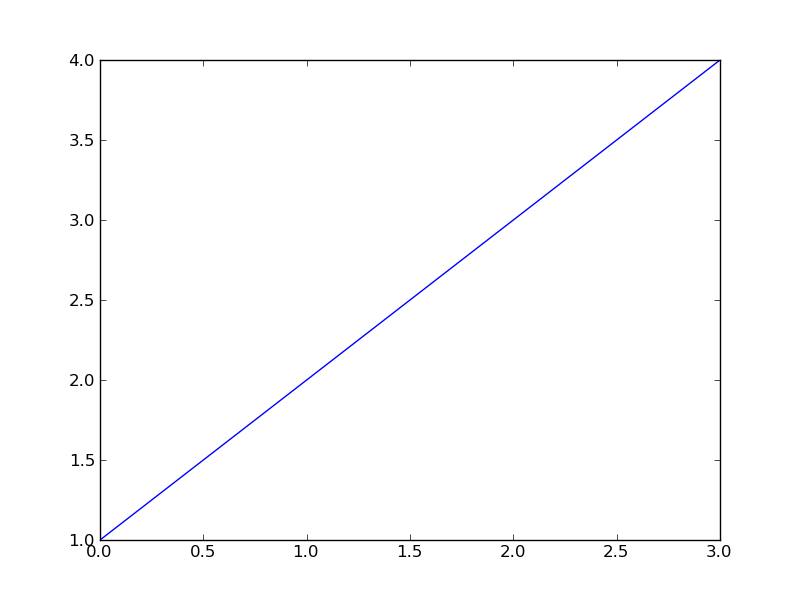
\includegraphics{figure1.png}
\caption{This is the caption. \label{egfig}}
\end{figure}

\begin{figure}
\centering
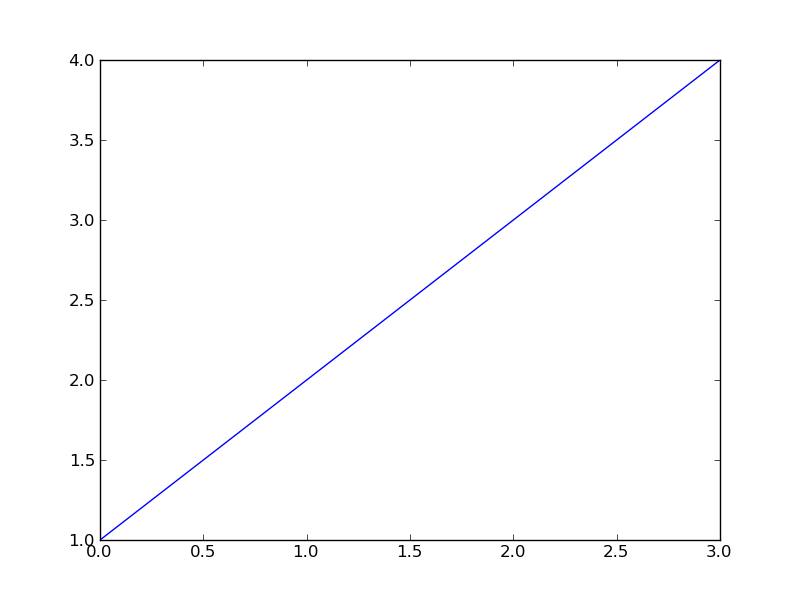
\includegraphics{figure1.png}
\caption{This is the caption on a smaller figure that will be placed by
default at the bottom of the page, and failing that it will be placed
inline or at the top. Note that for now, scale is relative to a
completely arbitrary original reference size which might be the original
size of your image - you probably have to play with it. \label{egfig2}}
\end{figure}

As you can see in Figures \ref{egfig} and \ref{egfig2}, this is how you
reference auto-numbered figures.

\begin{longtable}[]{@{}
  >{\raggedright\arraybackslash}p{(\columnwidth - 2\tabcolsep) * \real{0.1806}}
  >{\raggedright\arraybackslash}p{(\columnwidth - 2\tabcolsep) * \real{0.2361}}@{}}
\caption{This is the caption for the materials table.
\label{mtable}}\tabularnewline
\toprule\noalign{}
\begin{minipage}[b]{\linewidth}\raggedright
Material
\end{minipage} & \begin{minipage}[b]{\linewidth}\raggedright
Units
\end{minipage} \\
\midrule\noalign{}
\endfirsthead
\toprule\noalign{}
\begin{minipage}[b]{\linewidth}\raggedright
Material
\end{minipage} & \begin{minipage}[b]{\linewidth}\raggedright
Units
\end{minipage} \\
\midrule\noalign{}
\endhead
\bottomrule\noalign{}
\endlastfoot
Stone & 3 \\
Water & 12 \\
Cement & \(\alpha\) \\
\end{longtable}

We show the different quantities of materials required in Table
\ref{mtable}.

Unfortunately, restructuredtext can be picky about tables, so if it
simply won't work try raw LaTeX:

\begin{longtable}{lrrr}
\caption{Area Comparisons \label{quanitities-table}}
\tabularnewline
\toprule
\multirow{2}{*}{Projection} & \multicolumn{3}{c}{Area in square miles}\tabularnewline

& Large Horizontal Area & Large Vertical Area & Smaller Square Area\tabularnewline
\hline
Albers Equal Area  & 7,498.7 & 10,847.3 & 35.8\tabularnewline
Web Mercator & 13,410.0 & 18,271.4 & 63.0\tabularnewline
Difference & 5,911.3 & 7,424.1 & 27.2\tabularnewline
Percent Difference & 44\% & 41\% & 43\%\tabularnewline
\bottomrule

\end{longtable}

Perhaps we want to end off with a quote by Lao Tse\footnote{\(\mathrm{e^{-i\pi}}\)}:

\begin{quote}
\emph{Muddy water, let stand, becomes clear.}
\end{quote}

\hypertarget{customised-latex-packages}{%
\section{Customised LaTeX packages}\label{customised-latex-packages}}

Please avoid using this feature, unless agreed upon with the proceedings
editors.

\bibliography{mybib}
\bibliographystyle{ieeetr}

\end{document}